\subsection{FFS - Forces on Fracture Surfaces}
\label{chap:NumPlatf:FFS}
\begin{figure}[htb!]
\begin{center}
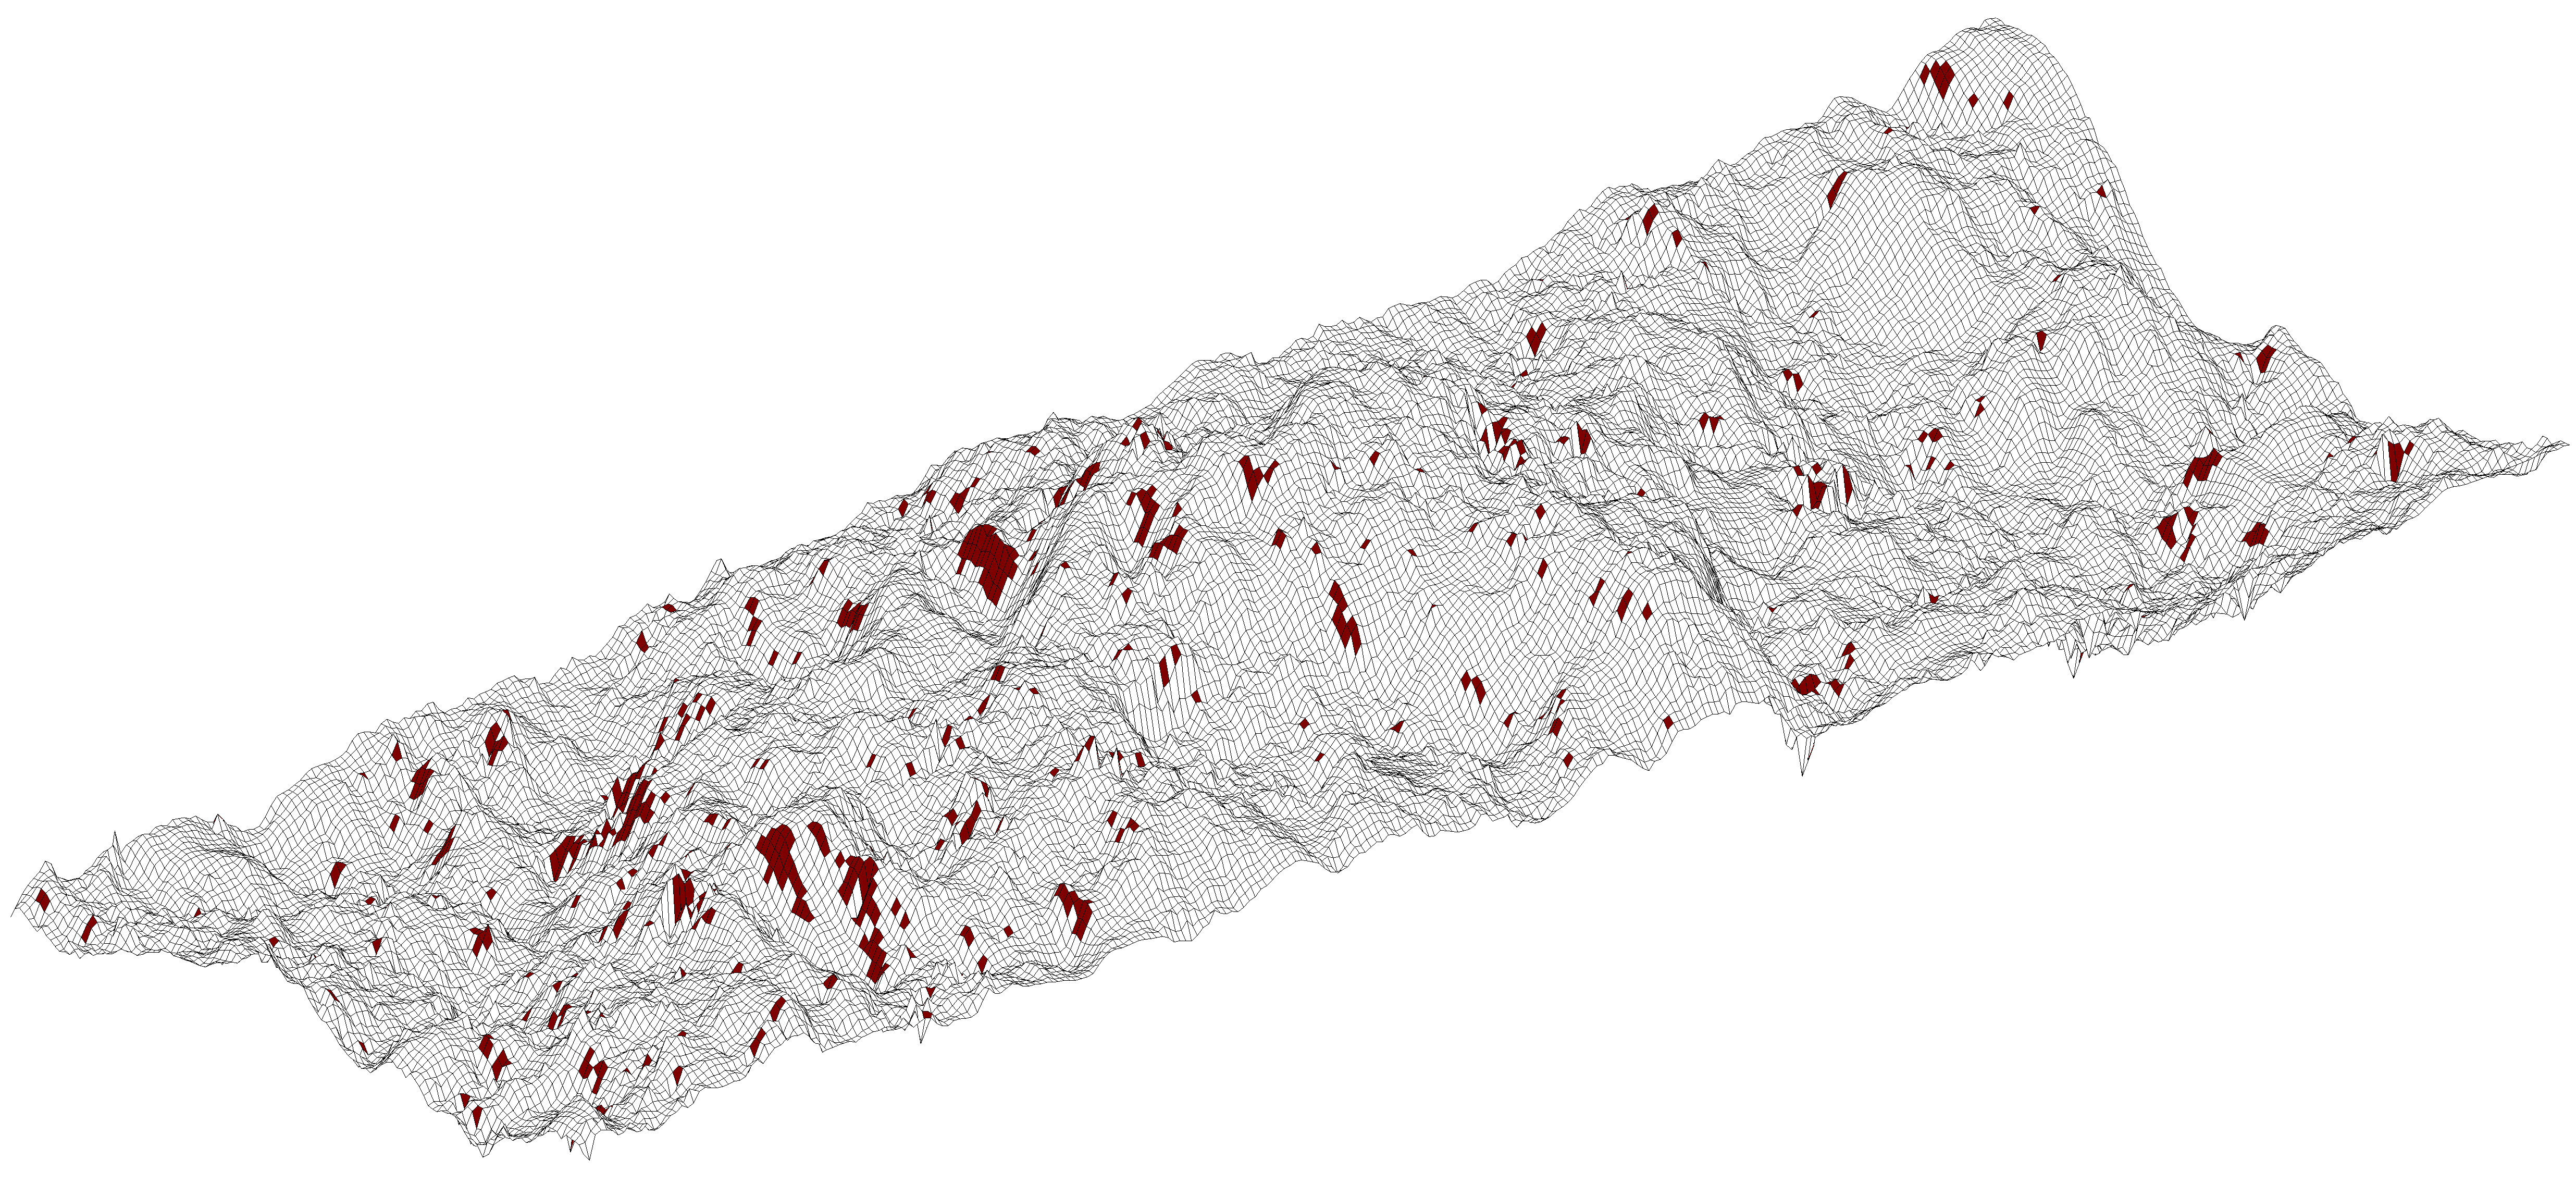
\includegraphics[width=0.6\textwidth]{./figures/FFS_MarkedSurfaceElements.png}
\end{center}
\caption{The elements used in a shear test simulation are marked in red. The FFS approach is able to look directly inside a model and helps to deepen the understanding of the active processes.}
\label{Fig:FFS-MarkedElements}
\end{figure}
This numerical method explicitly uses the geometry of a rock surface and calculations on single surface elements are executed. The main advantage of this method is the possibility to closely look inside the mechanisms which control the shear behaviour of the joint (Figure \ref{Fig:FFS-MarkedElements}). The drawback is the high computation time needed due to the more complex calculation scheme.\\
Starting point were the works by \cite{Fathi2016} and \cite{Casagrande2017}. The last mentioned work uses a FFS approach. The geometry of surface is represented as a triangular surface. The apparent dip angles $\theta^\ast$ for the elements are calculated. An iterative scheme decides whether the surface can slide over its counterpart or whether the surface elements in contact are destroyed. In the case of destruction the geometry is corrected and the next check for sliding versus destruction starts. The two important formulas are the one for the sliding forces: 
\begin{equation}
F_{slide}=F_{loc} \cdot \tan (\varphi_b + \theta^\ast)
\end{equation}
where $F_{loc}$ is the local force acting on one element, $\Phi_b$ is the basic friction and $\theta^\ast$ the apparent dip angle of this element.\\
The other formula is the one for shear forces, which is the force needed to destroy the surface element:
\begin{equation}\label{eq:shear}
F_{shear}=A \cdot (c + \sigma_{loc}*tan(\Phi))
\end{equation}
where $A$ is the ground area of the element, $c$ the cohesion of the rock material, $\sigma_{loc}$ the local normal stress and $\Phi$ the angle of inner friction of the rock material.



\begin{figure}[htb!]
\begin{center}
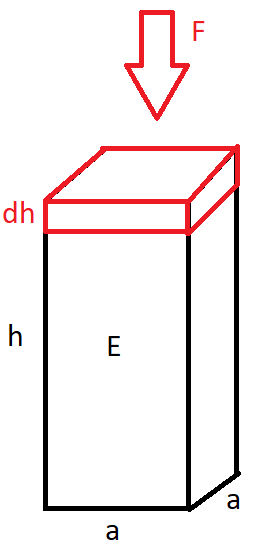
\includegraphics[width=0.2\textwidth]{./figures/FFS_NormalForce.png}
\end{center}
\caption{A surface element is represented as a rock column which with\-stands normal forces by elastic deformation.}
\label{Fig:FFS-NormalForce}
\end{figure}
The idea of the newly developed approach is to have a physically consistent calculation scheme. Therefore the normal forces of the surface elements in contact have to be estimated. The simplest approach was chosen to keep things manageable. An elastic stress-displacement behaviour was basically used (Figure \ref{Fig:FFS-NormalForce}). The resulting formula is:
\begin{equation}
F_n= \sum_i E * a^2 * \frac{\Delta h_i}{h}
\end{equation}
For all $i$ surface elements in contact the relative height change $\frac{\Delta h}{h_i}$, the ground area $a^2$ and the Young's modulus $E$ were used. For a specific rock joint the two surfaces are moved towards each other until the force created by the elastic deformation equals the force which is applied to the fracture.\\
\ \\
Another simplification compared to \cite{Casagrande2017} is the usage of quadratic grid elements. This allows to store the height values in a matrix form which is easy to handle.  